\chapter{二维材料异质结生长机理的研究}
\section{引言}
石墨烯作为经典的二维材料,由于独特的晶体结构和电子结构特性,在超导,量子计算、量子晶体管等方面具有独特的优势\citing{RN1068-2020,RN1071-2021,RN1065-2013,RN997-2007,RN1008-2015}。而要将石墨烯与现行集成电路使用的平面硅工艺兼容,需要将石墨烯转移到\cemb{SiO2}等绝缘衬底的表面。而石墨烯在\cemb{SiO2}等绝缘衬底表面通常以无序的状态存在,破碎的晶格使得石墨烯在这些绝缘衬底的表面难以完全发挥出理论上限。

而作为二维材料中的绝缘体,六方氮化硼\cemb{h-BN}在具有较大的带隙的同时也保有二维材料高质量面内结构的特点。趋近完美的二维晶体结构使得\cemb{h-BN}在禁带内具有极低的缺陷态密度以及较高的击穿电压。同时,\cemb{h-BN}与石墨烯之间的晶格失配只有\SI{2}{\percent},这使得\cemb{h-BN}非常适合搞高性能电子器件中替代\cemb{SiO2}作为石墨烯的衬底材料 \citing{RN959-2010}。这种将不同的二维材料纵向堆叠起来可以制成纵向异质结,层与层之间由较弱的范德华力或准范德华力连接。以二维材料所组成的异质结能够结合不同二维材料优异的物理特性,使得二维材料在多种新型器件中能够最大化的发挥其独特的优势。许多新奇的物理现象已经在石墨烯和\cemb{h-BN}的纵向堆叠而成的二维异质结被研究者所发现,如在外磁场下电子和磁场场强的霍夫斯塔特蝴蝶分型图像\citing{RN1286-2013, RN1287-2013, RN1285-2013}。同时,石墨烯/\cemb{h-BN}纵向二维异质结具有非常好的制备质量,石墨烯高度可调的物理特性,以及二者之间存在的周期性的摩尔超晶格。这些都使得石墨烯/\cemb{h-BN}纵向二维异质结成为了一个非常好的观测新奇量子现象的基础平台。

然而,虽然机械剥离的方式能够制备具有极高质量的石墨烯/\cemb{h-BN}纵向二维异质结,但受限于较低生产效率和高昂的合成成本,剥离的方式很难应用于大规模的二维材料的生产制备。而常用于大规模低成本制备石墨烯的化学气相沉积法通常需要\cemb{Cu}等金属衬底的催化作用的协助。由于\cemb{h-BN}对于甲烷等含碳前驱体裂解反应的催化活性远不及金属衬底,石墨烯在\cemb{h-BN}上直接生长的速率同样也远低于在金属衬底上的生长速率。因此,一些研究者试图通过增加前驱体裂解速率的方式提升纵向二维异质结的合成效率。例如,在2013年,研究者发现通过等离子体辅助的方式能够在低温的环境下在\cemb{h-BN}的表面生长石墨烯\citing{RN1289-2013}。在2015年,研究者通过添加作为气体催化剂的硅烷等方式,可以促进甲烷的裂解,提高石墨烯在\cemb{h-BN}表面的生长速率\citing{RN1059-2015}。但以上方式通常使用剥离的\cemb{h-BN}作为石墨烯的生长衬底,使用较高的生长温度或者使用等离子体辅助的方式进行生长。在这种情况下,虽然石墨烯能够在\cemb{h-BN}的表面生长,但是高温会破坏金属衬底,而\cemb{h-BN}本身的生长需要在金属衬底的表面。因此我们需要寻找到一种生长流程,使得温度维持在金属衬底能够生长\cemb{h-BN}能够的同时,尽可能的加快石墨烯在\cemb{h-BN}表面的生长速率。

在\ref{cap:CG}章中,我们构建了一种利用\cemb{Cu}蒸气近邻催化效应在\cemb{h-BN}表面直接堆叠生长石墨烯的方法。该方法利用从外缘\cemb{Cu}源处蒸发而出的\cemb{Cu}蒸气作为催化剂,在\cemb{h-BN}的表面产生对\cemb{CH4}的近邻催化效应,加速甲烷在\cemb{h-BN}表面的裂解,从而达到加速\cemb{h-BN}表面石墨烯生长的目的。利用理论计算的方法,我们证明了\cemb{Cu}蒸气从蒸发源到达\cemb{h-BN}表面并进行\cemb{CH4}裂解催化的可行性,同时给出了裂解而成的碳原子在\cemb{h-BN}表面成核生长成石墨烯的生长序列。我们认为通过这种直接堆叠生长的方法能够能够实现石墨烯/\cemb{h-BN}的双层以及多层堆叠交替大规模生长,进一步提升石墨烯/\cemb{h-BN}二维纵向异质结在高性能电子器件应用的可行性,推进石墨烯/\cemb{h-BN}二维纵向异质结的工程化和集成化。

\section{计算细节}

在本章中密度泛函理论主要使用Vienna ab-initio Simulation Package (VASP) 软件包进行计算。在密度泛函理论计算中,我们使用广义梯度近似(GGA)下的 Perdew-Burke-Ernzerhof (PBE)泛函描述电子之间的交换关联作用。平面波的截断动能取为为$\SI{500}{\electronvolt}$。为了研究\cemb{Cu}/\cemb{h-BN}衬底表面石墨烯的生长情况,我们采用切片模型并在垂直表面方向放置至少$\SI{20}{\angstrom}$的真空层以防止周期性条件相邻切片的影响。切片模型中,作为石墨烯生长衬底的\cemb{Cu}/\cemb{h-BN}包含四原子层的\cemb{Cu(111)}以及单原子层的\cemb{h-BN}。在\cemb{Cu}的表面,经过我们的计算,\cemb{h-BN}的最优堆叠方式为\cemb{N}原子位于\cemb{Cu}衬底的顶位,\cemb{B}原子位于\cemb{Cu}衬底的面心立方位(fcc site)。
在原子结构优化的计算中,力收敛条件设为$\SI{2e-2}{\electronvolt \per \angstrom}$,电子结构自洽场计算的收敛条件设为$\SI{1e-6}{\electronvolt}$。
对于碳团簇(\cemb{C_x})、石墨烯、\cemb{h-BN}、\cemb{Cu}衬底之间之间的范德瓦尔斯作用使用Grimme的DFT-D3方法进行描述,并带有Becke-Johnson阻尼作用 \citing{RN937-2010, RN938-2011}。
对于过渡态的计算,我们采用CI-NEB(Climbing Image Nudged Elastic Band)方法对始末反应状态之间的能量鞍点进行搜寻,以确定反应势垒的大小\citing{RN790-2000}。对于过渡态计算,力收敛条件设为$\SI{3e-2}{\electronvolt \per \angstrom}$。

\section{石墨烯/\cemb{h-BN}纵向二维异质结的生长机理}
    \label{cap:CG}
    图\ref{fig:CG_diagram_routine}和图\ref{fig:CG_diagram_growthSketch}为我们设计的利用\cemb{Cu}蒸气近邻催化效应在\cemb{h-BN}表面直接堆叠生长石墨烯的装置示意图和生长机理示意图。首先,我们可以在下方的\cemb{Cu}衬底表面利用常规的低压化学气相沉积法大面积的生长\cemb{h-BN}。这里我们使用液态环硼氮烷(borazine)作为生长前驱体。下方的加热器为\cemb{h-BN}大面积生长时提供合适的生长温度。当\cemb{h-BN}覆盖满下方\cemb{Cu}衬底的表面时,我们在上上方的加热器处引入第二片\cemb{Cu}源用于蒸发产生\cemb{Cu}蒸气。蒸发开始了额一段时间之后,\cemb{Cu}蒸气在扩散作用下充满\cemb{h-BN}上方的空间,此时引入甲烷\cemb{CH4}作为石墨烯生长的前驱体,通过调整\cemb{h-BN}和上方铜蒸发源之间的距离至合适的位置,我们就可以在下方\cemb{Cu}表面的已生长\cemb{h-BN}的表面直接堆叠生长石墨烯。需要注意的是,由于作为前驱体的甲烷\cemb{CH4}直接通入衬底和蒸发源之间的间隙,因此会在上方\cemb{Cu}蒸发源的表面形成石墨烯,当石墨烯覆盖满上方的\cemb{Cu}蒸发源的表面后,\cemb{Cu}蒸发源将会失去产生原有的\cemb{Cu}蒸气的能力,无法继续为\cemb{h-BN}表面甲烷的裂解提供气态催化剂。这时需要通过机械装置(图\ref{fig:CG_diagram_routine})替换掉已经蒸发能力衰减的\cemb{Cu}蒸发源,利用新换上的表面无石墨烯的\cemb{Cu}蒸发源继续提供\cemb{Cu}蒸气在\cemb{h-BN}表面生长石墨烯。

    \begin{figure}[htb]
        \subfloat[]{
            \centering
            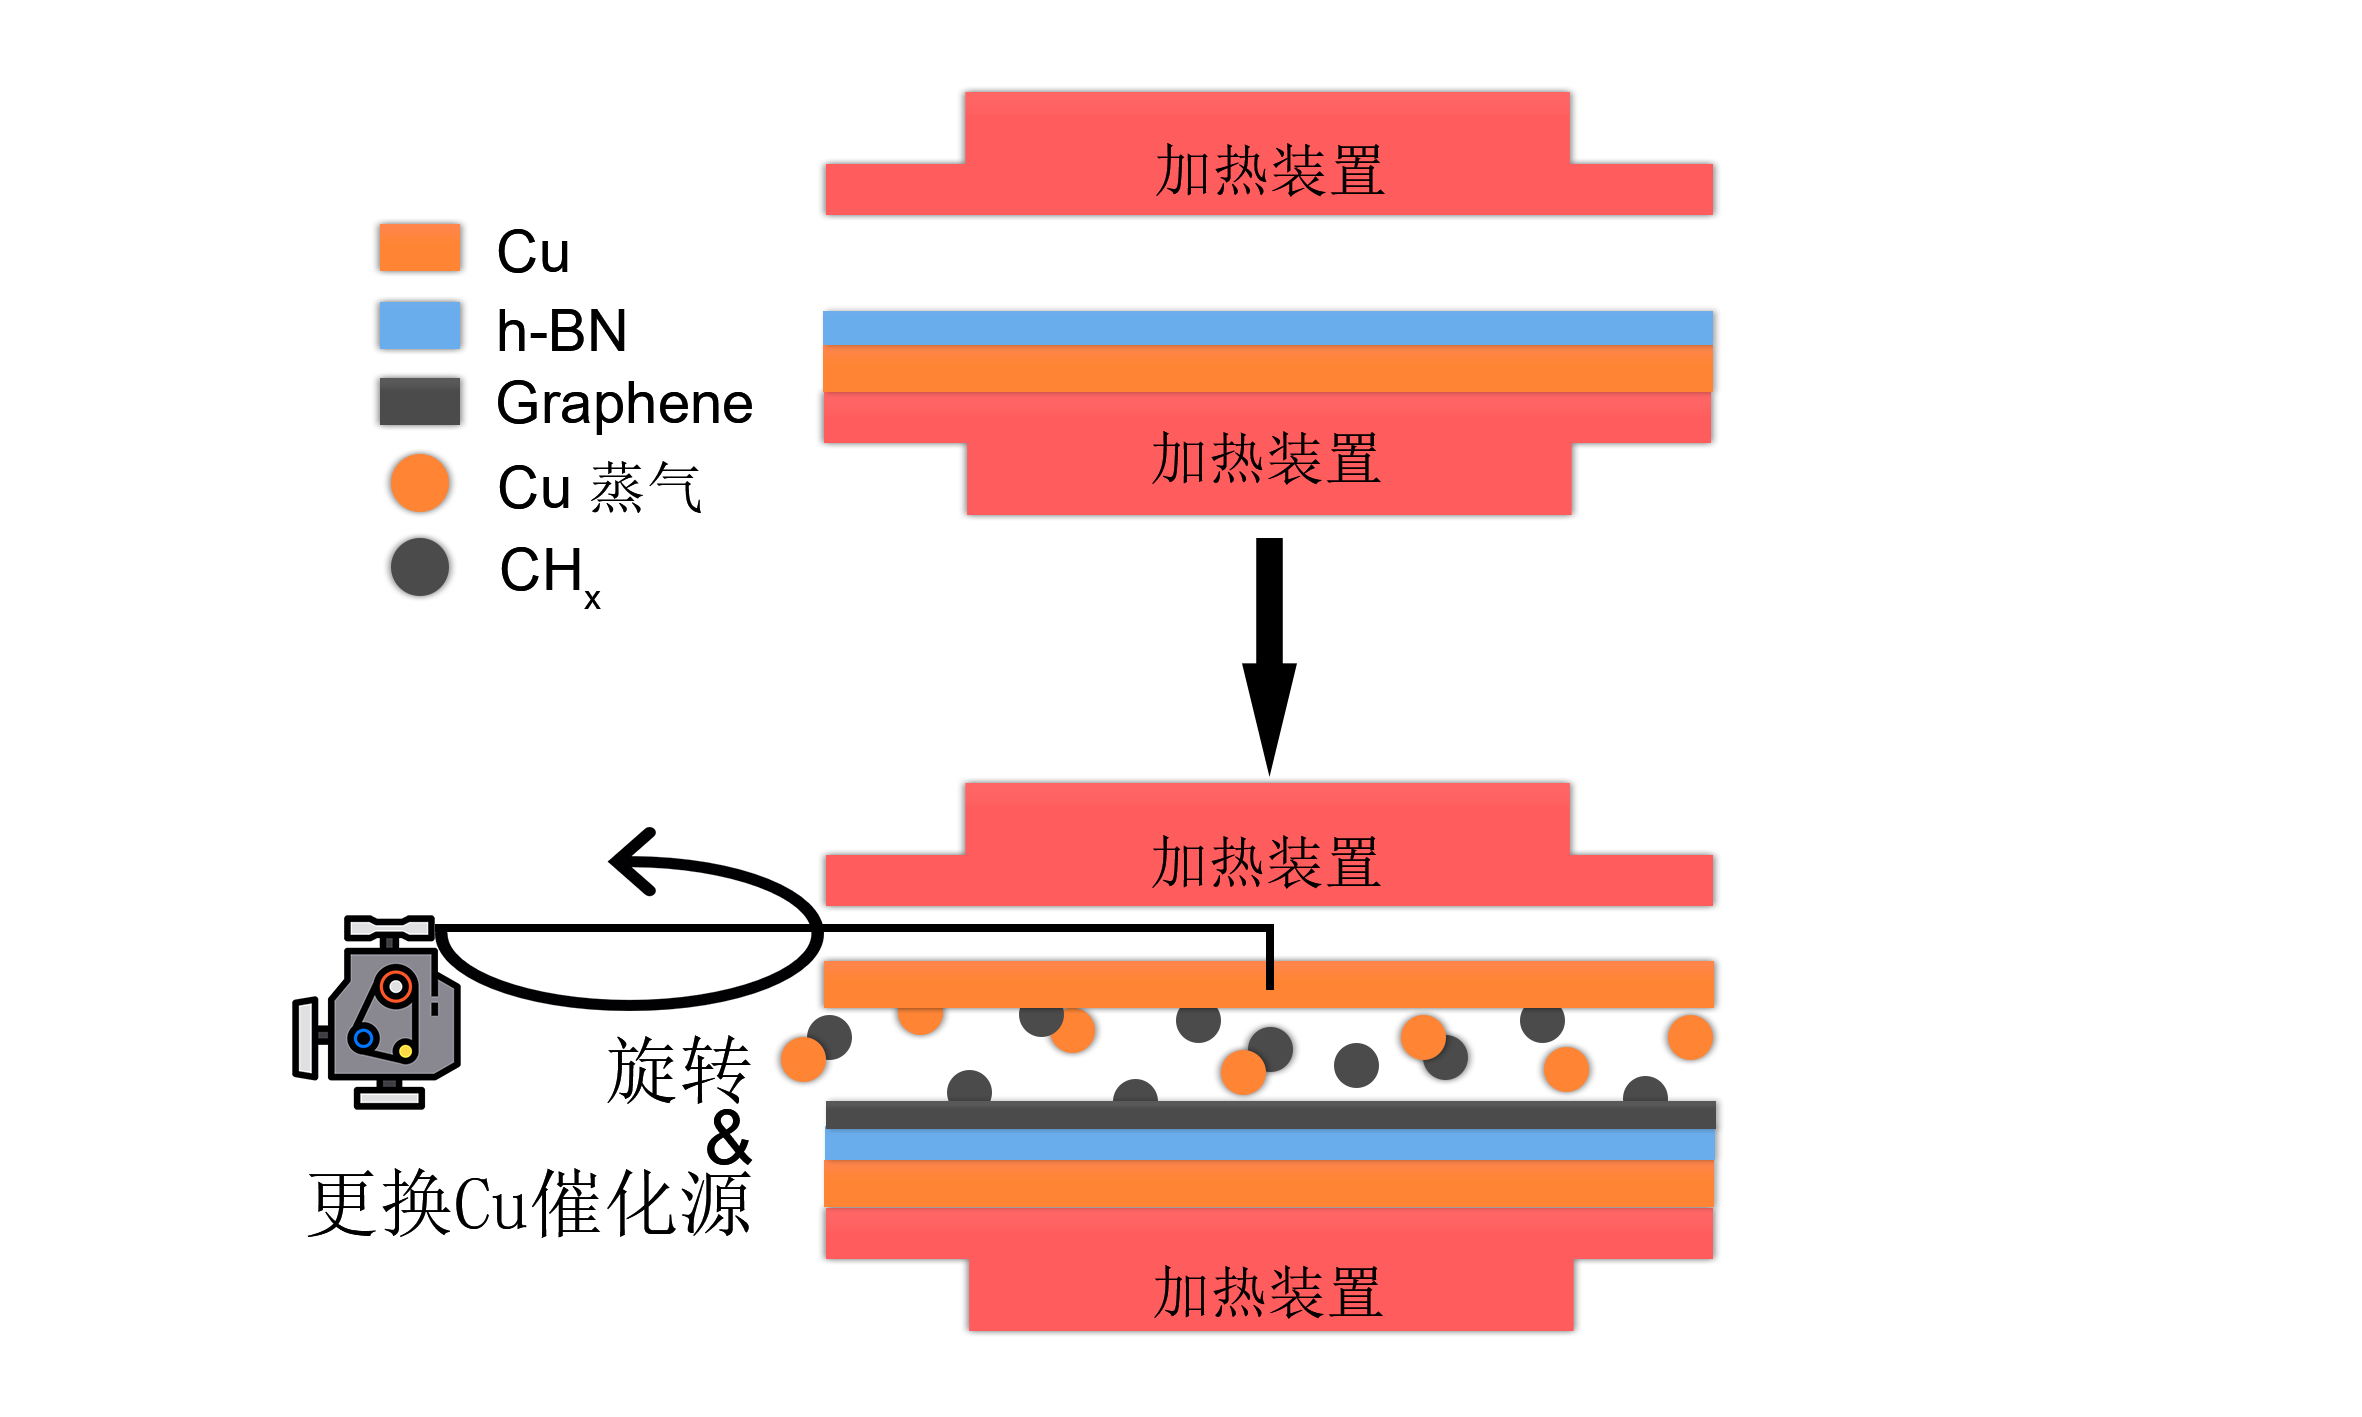
\includegraphics{pic/CG_diagram_routine.png}
            \label{fig:CG_diagram_routine}
        }
        \newline
        \subfloat[]{
            \includegraphics{pic/CG_diagram_growthSketch.png}
            \label{fig:CG_diagram_growthSketch}
        }
        \caption{利用\cemb{Cu}蒸气近邻催化效应在\cemb{h-BN}表面直接堆叠生长石墨烯。(a)生长装置示意图;(b)石墨烯/\cemb{h-BN}异质结生长过程示意图}
        \label{fig:CG_diagram_CVD}
    \end{figure}

    \subsection{近邻蒸发气态\cemb{Cu}催化剂的扩散}
    
    事实上,在\cemb{h-BN}上方的\cemb{Cu}蒸发源对于石墨烯在\cemb{h-BN}表面的直接石墨烯生长可能纯在两种作用\chinesecolon 一种是如上文所说的,\cemb{Cu}蒸发源的表面蒸发出浓度较高的\cemb{Cu}蒸气,这些\cemb{Cu}蒸气在扩散至\cemb{h-BN}表面仍然能够保持较高的浓度和分压。随后在\cemb{Cu}蒸气的催化作用下,生长气氛中的\cemb{CH4}逐渐脱氢裂解为活性碳原子\cemb{C},在\cemb{h-BN}表面成核生长成为石墨烯。另一种方式是\cemb{CH4}直接在\cemb{Cu}的表面脱氢裂解,产生的活性碳原子(\cemb{C})和活性碳氢化合物(\cemb{CH})等基团在热动能的作用下脱离\cemb{Cu}铜蒸发源的表面,扩散至下方\cemb{h-BN}的表面进行成核、生长石墨烯。

    为了判定并且验证在\cemb{h-BN}表面生长石墨烯的生长机制,我们首先使用自由分子流模拟\cemb{Cu}蒸发源产生的\cemb{Cu}蒸气在扩散至\cemb{h-BN}表面后的浓度。图\ref{fig:CG_diagram_FEM_structure}为我们所构建的在自由分子流模型下\cemb{Cu}蒸气产生和扩散的模拟结构图。我们考虑圆盘形的\cemb{Cu}衬底和\cemb{Cu}蒸发源,半径为\SI{500}{\micro\meter}。\cemb{Cu}蒸发源悬挂在\cemb{Cu}衬底和\cemb{h-BN}的上方,间隔一定距离。\cemb{Cu}蒸发源的温度设置为\SI{1200}{\kelvin},此时蒸发出的\cemb{Cu}蒸气的饱和蒸汽压约为\SI{1.25E-13}{\pascal}。对于蒸发出的\cemb{Cu}蒸气,我们只关注从蒸发源下表面蒸发出的\cemb{Cu}原子流,并且遵循朗缪尔蒸发公式(Langmuir’s Equation of evaporation)。
    
    \begin{figure}[htb]
        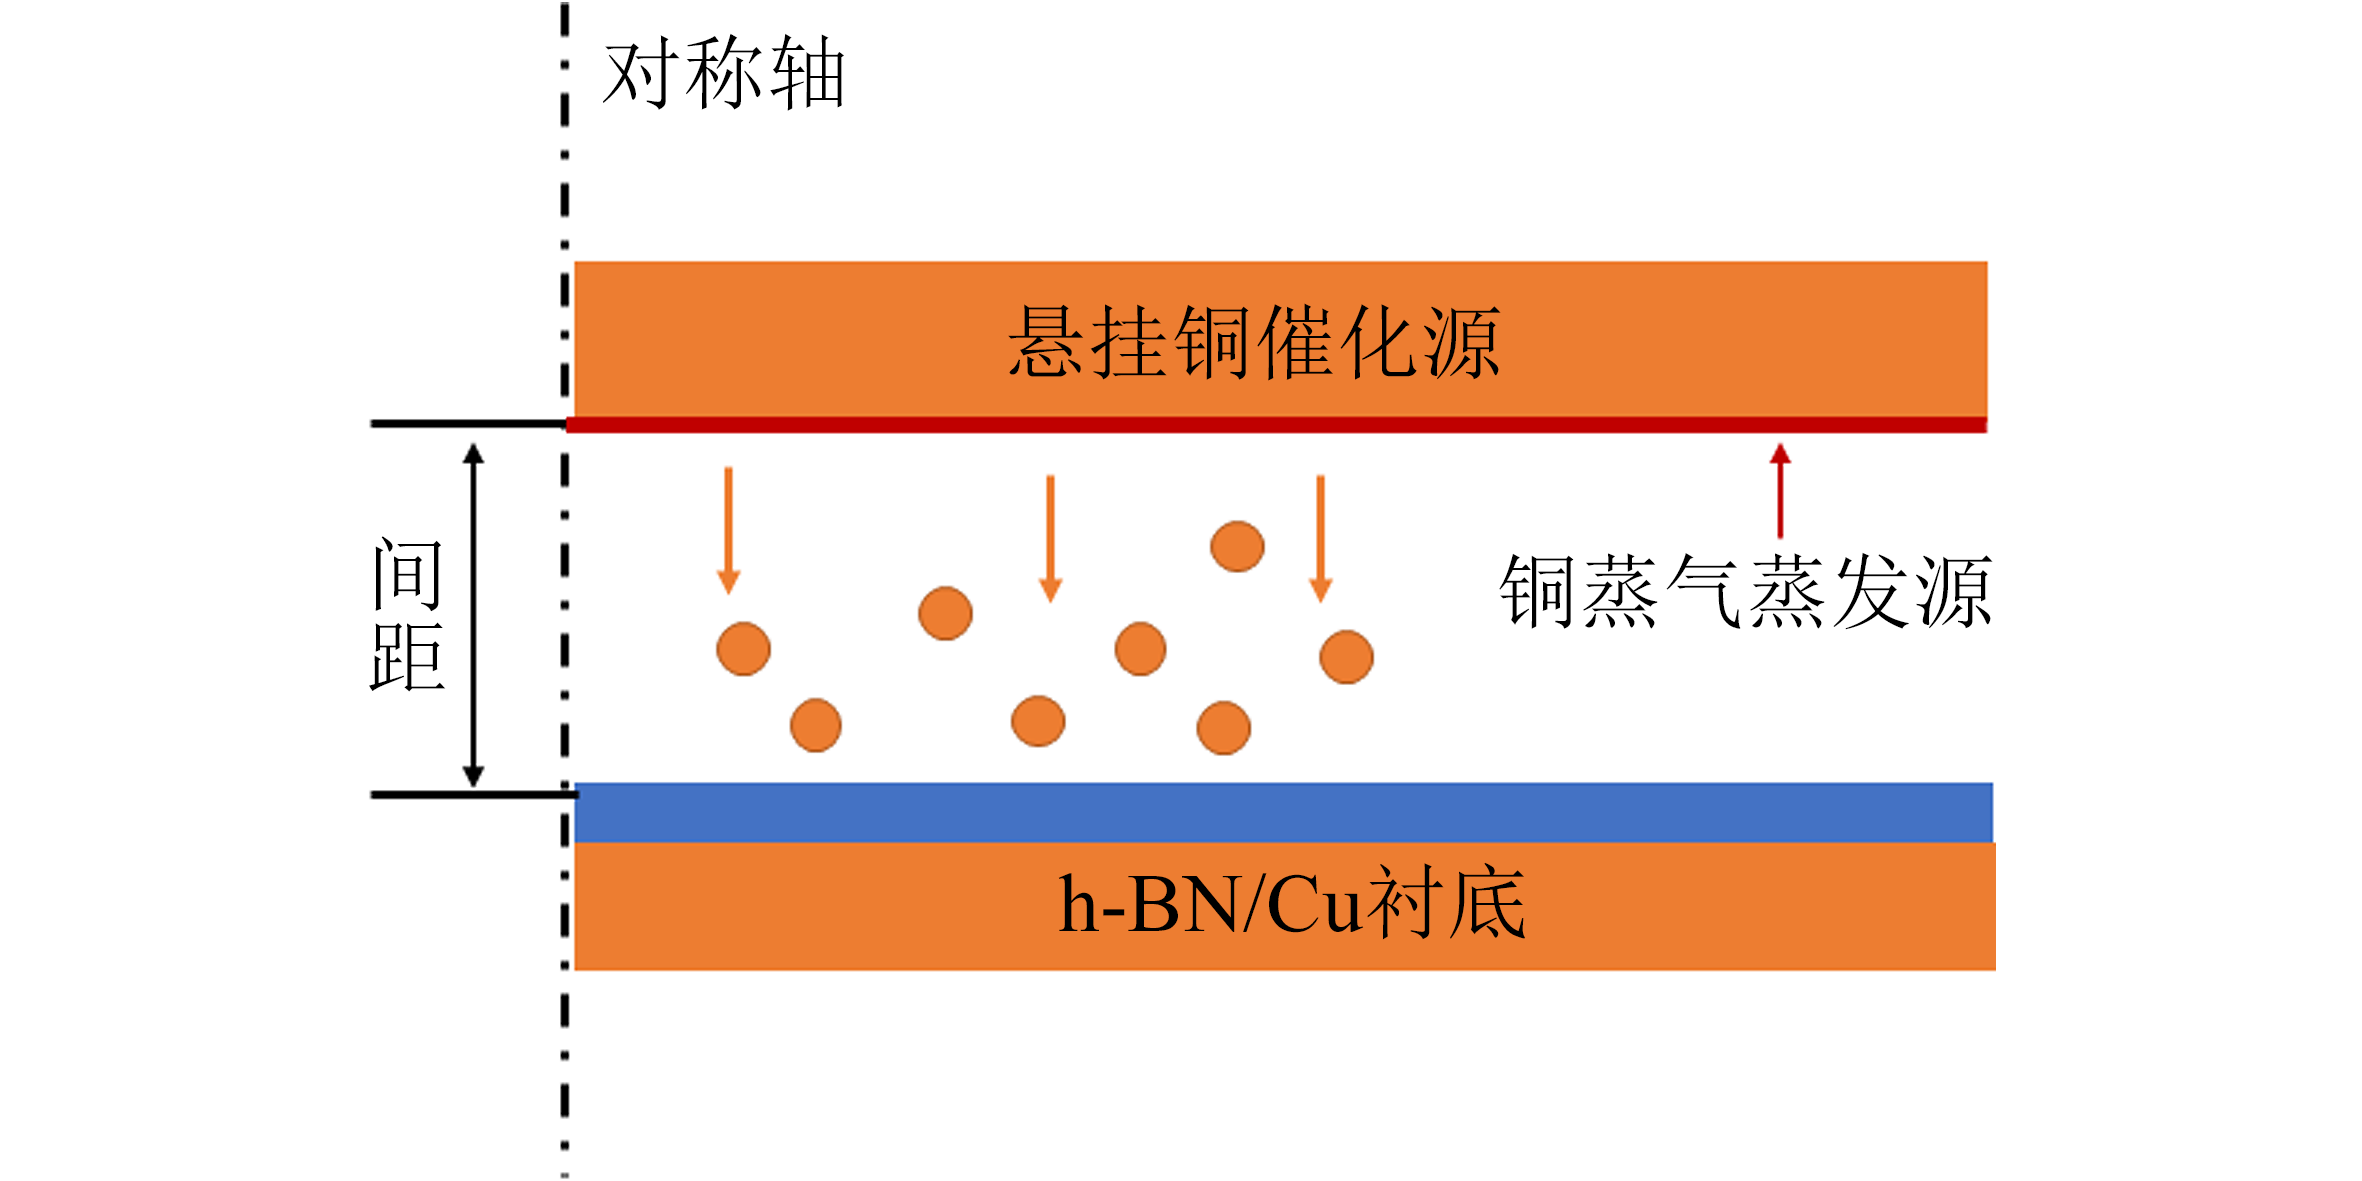
\includegraphics{pic/CG_diagram_FEM_structure.png}
        \caption{化学气相沉积腔体内\cemb{Cu}蒸气扩散模拟示意图。}
        \label{fig:CG_diagram_FEM_structure}
    \end{figure}

    使用自由分子流模拟,我们首先研究上方的\cemb{Cu}蒸发源未被石墨烯覆盖的情况。在图\ref{fig:CG_FEM_fullCu}中我们绘制了蒸发源和\cemb{Cu/h-BN}表面的距离在$\SI{4}{\micro\meter} \sim \SI{100}{\micro\meter}$的时候和,蒸发至下方\cemb{Cu/h-BN}表面的\cemb{Cu}蒸气的气压分布情况。可以看到对于\cemb{Cu/h-BN}表面,即使上方\cemb{Cu}蒸发源的距离从\SI{4}{\micro\meter}扩大至\SI{100}{\micro\meter}其的中心处的\cemb{Cu}蒸气的气压略微下降,接近于蒸发温度下的\cemb{Cu}原子的饱和蒸汽压\SI{1.25}{\pascal}。当\cemb{Cu}蒸发源和\cemb{Cu/h-BN}之间的距离很近时,\cemb{Cu/h-BN}表面\cemb{Cu}蒸气的气压随着半径的衰减很小,只在接近边缘的位置由于\cemb{Cu}蒸气的向外扩散,导致\cemb{Cu/h-BN}表面边缘处(半径$\geqslant \SI{400}{\micro\meter}$)出现了\cemb{Cu}蒸气气压的明显下降。当\cemb{Cu}蒸发源和\cemb{Cu/h-BN}的距离扩大时,在\cemb{Cu/h-BN}表面\cemb{Cu}蒸气气压随着半径的衰减作用变强。当二者的距离提高到\SI{100}{\micro\meter}时,在\cemb{Cu/h-BN}表面半径为\SI{300}{\micro\meter}位置就已经可以观察到较为明显的\cemb{Cu}蒸气气压下降。当\cemb{Cu}蒸发源未被石墨烯覆盖的时候,在\cemb{Cu/h-BN}表面最外缘处(\SI{500}{\micro\meter})的\cemb{Cu}蒸气气压随与\cemb{Cu}蒸发源之间距离的上升而下降的驱使不明显。当距离为\SI{4}{\micro\meter}时,\cemb{Cu/h-BN}表面最外缘处的\cemb{Cu}蒸气气压为\SI{8e-4}{\pascal}。而当距离扩展到\SI{100}{\micro\meter}时,在\cemb{Cu/h-BN}表面最外缘处仍可以保持大约\SI{6e-4}{\pascal}的\cemb{Cu}蒸气。

    \begin{figure}[htb]
        \includegraphics{pic/CG_FEM_fullCu.png}
        \caption{不同间距下\cemb{Cu/h-BN}表面\cemb{Cu}蒸气的气压分布情况。}
        \label{fig:CG_FEM_fullCu}
    \end{figure}

    当在\cemb{Cu/h-BN}的表面生长了一段时间的石墨烯后,由于\cemb{CH4}在\cemb{Cu}蒸发源的表面同样会裂解沉积生长石墨烯,\cemb{Cu}蒸发源会有部分表面覆盖上新生长的石墨烯而从而失去蒸发\cemb{Cu}蒸气的能力。考虑到石墨烯生长前驱体\cemb{CH4}通常来自\cemb{Cu}蒸发源外部的气流,因此我们简单的将\cemb{Cu}蒸发源表面随着生长过程进行而生长的石墨烯限制在\cemb{Cu}蒸发源圆盘的外缘。在图\ref{fig:CG_FEM_halfCu}中,我们模拟了在被石墨烯覆盖了外半圈\cemb{Cu}蒸发源的情况下,扩散至\cemb{Cu/h-BN}表面\cemb{Cu}蒸气的气压分布情况。可以看到相比于完整的\cemb{Cu}蒸发源,被石墨烯覆盖的\cemb{Cu}蒸发源只能在
    %//TODO

    \begin{figure}[htb]
        \includegraphics{pic/CG_FEM_halfCu.png}
        \caption{不同间距下\cemb{Cu}蒸发源的外半圈被石墨烯覆盖后蒸发、扩散至\cemb{Cu/h-BN}表面的\cemb{Cu}蒸气的气压分布情况。}
        \label{fig:CG_FEM_halfCu}
    \end{figure}
    \begin{figure}[htb]
        \includegraphics{pic/CG_FEM_fullCuCenterVariousDistance.png}
        \caption{}
        \label{}
    \end{figure}

    \subsection{气态\cemb{Cu}催化剂对甲烷裂解反应的催化性能}
    \subsection{\cemb{h-BN}表面石墨烯的生长演化机理}
\section{石墨烯/二硒化钒横向异质结的生长机理}
\section{总结}